% !TEX root =  mosaic.tex
\section{Background and Motivation}
\label{sec:background}

This section introduces the background and the GPU-specific challenges behind analytical selection.

\subsection{GPU Execution Space Decisions}
\label{sec:bg-decisions}
\label{sec:gpu-execution-model}

A GPU kernel launches a grid of thread blocks; each block runs on an SM whose resident-block count is limited by block/thread limits, per-block shared memory, and per-thread registers. \name targets the execution space decisions that set these quantities: tile sizes, thread block dimensions, thread mappings, shared memory placement, and register blocking. Larger tiles improve reuse but grow footprint and live state, while smaller tiles raise occupancy but expose less locality. As each tile or placement choice moves several of these limits at once, they cannot be treated as independent dials.

\name does not perform transformation scheduling. It starts from a transformed program whose legal order is fixed by an existing scheduler: schedule trees and affine accesses for polyhedral compilers~\cite{ppcg,tc}, or schedule traces and tensor metadata for template compilers~\cite{halide,tvm}. From this representation, \name extracts loop extents, schedule annotations, access footprints, read/write polarity, operation counts, and coalescing layout, enough to classify dimensions and array roles without depending on compiler internals.


%\subsection{Why Execution Space Parameters Matter}
%\label{sec:bg-why}
%\label{sec:execution space-motivation}

To make the case concrete, we hold one GEMM (general matrix multiplication) schedule fixed and sweep only its execution space parameters: tile sizes \((\tau_i,\tau_j)\), thread block shapes \((b_i,b_j)\), and shared memory placement. We construct 5,000 candidate configurations; 2,232 successfully launched, for which PPCG~\cite{ppcg} emitts each kernel and we measure execution time on an RTX 4090. \autoref{fig:motivation-landscape} plots the results.

\begin{figure}[htbp]
  \centering
  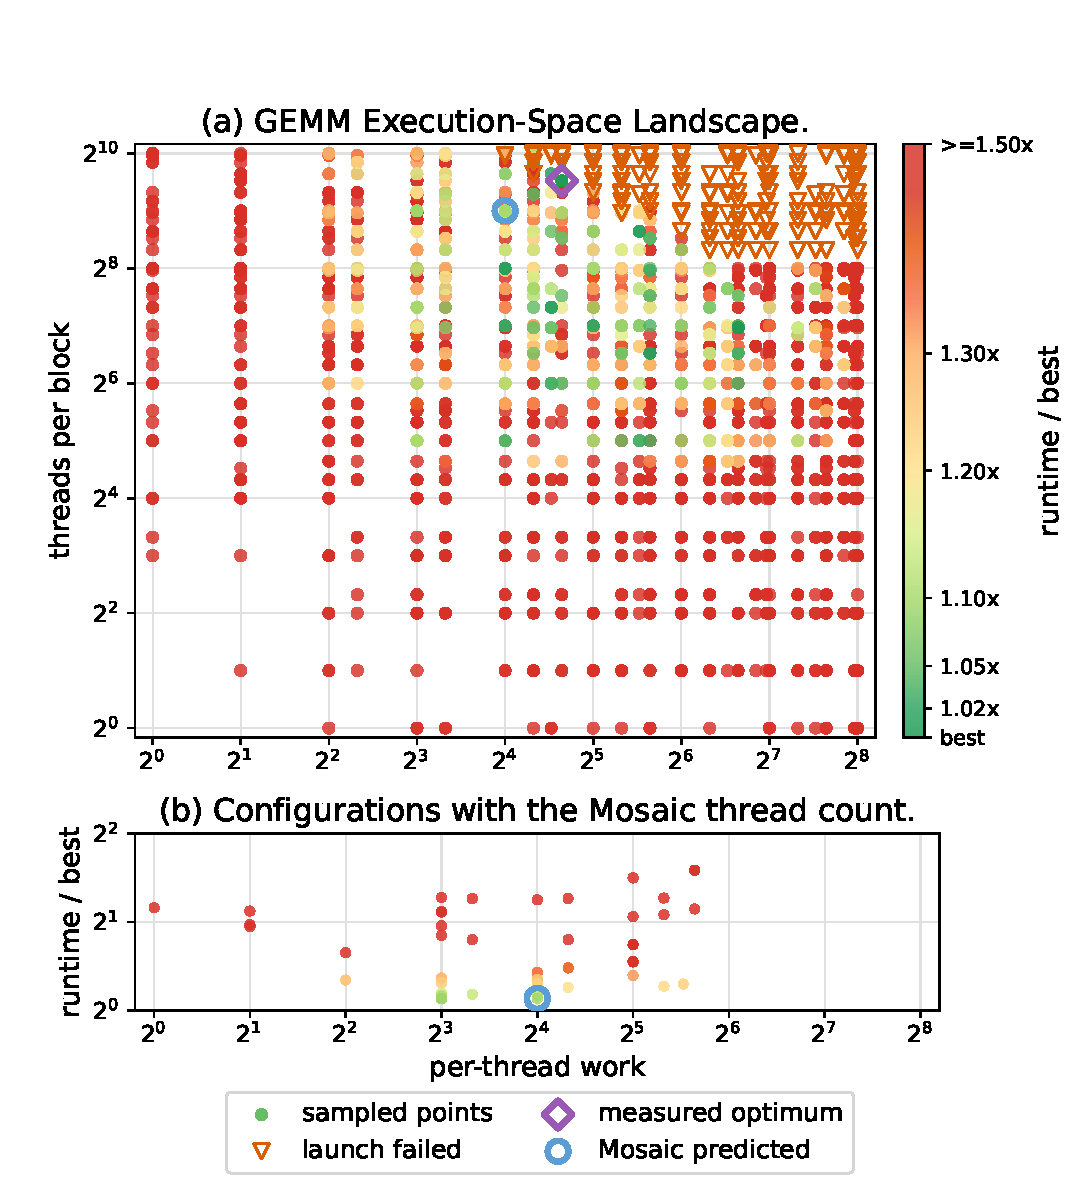
\includegraphics[width=\linewidth]{figure1_main.pdf}
  \caption{GEMM execution space landscape on RTX 4090 under a fixed schedule. (a) Log-ratio runtime for configurations that successfully launch, with measured and predicted optima marked. (b) One-dimensional slice at Mosaic's selected block-thread count, showing measured runtime as a function of per-thread work \(W=R_iR_j\).}
  \Description{Measured performance landscape for GPU GEMM execution space configurations.}
  \label{fig:motivation-landscape}
\end{figure}

\subsection{Transformation-Aware Program Representation}
\label{sec:bg-repr}
\label{sec:program-representation}

Under a single fixed schedule, execution space selection alone moves runtime by more than an order of magnitude, and only 28 of the 2,232 launched configurations (1.25\%) fall within 10\% of the best. Thus the choice of tile size, block shape, and placement, not the schedule, decides performance here. The surface in \autoref{fig:motivation-landscape}(a) is irregular and non-convex, and it shows that \name's analytical selection lands within 10\% of the measured optimum. \autoref{fig:motivation-landscape}(b) fixes the thread block size to the \name-selected block thread count and isolates how per-thread work \(W=R_iR_j\) affects the measured runtime. The slice shows that even after the thread block size is fixed, measured runtime varies substantially with \(W\), so register blocking remains a first-order execution space decision rather than a residual tie break.

\subsection{GPU-Specific Modeling Challenges}
\label{sec:bg-challenges}
\label{sec:gpu-modeling-challenges}

\label{sec:challenge-register-cycle}
\label{sec:challenge-placement}
\label{sec:challenge-discrete-objective}
\label{sec:challenge-register-pressure}

Analytical execution space optimization must address four GPU-specific challenges. First is an occupancy--register circular dependence: the per-thread register budget depends on the number of resident blocks and threads on an SM, yet the resident-block count itself depends in part on register usage, and an analytical model, unlike a tuner, cannot compile each candidate and read back achieved occupancy. Second, shared memory placement is coupled with tile selection: staging read-only operands cuts global traffic but consumes capacity and may lower the resident-block count, so the best placement depends on tile size, block shape, and reuse pattern and cannot be chosen before them. Third is discrete wave quantization: an SM hosts an integer number of blocks, so a grid executes in a discrete number of waves whose ceiling shifts with tile and placement choices, producing step boundaries that no static linear constraint or smooth objective captures. Finally, register pressure is unknown before code generation, because the exact register count is set by the backend allocator afterward, so a sound model needs a conservative compile-time feasibility filter.

The implication is that \emph{these four effects are not independent knobs but one coupled feedback loop}, in which footprint, resident blocks, register budget, and wave count all move together, so they must be resolved jointly in a single formulation rather than by a sequence of independent heuristics.
